\chapter{Marco te\'orico}\label{chap_main_files}
\minitoc

\section{Microscop\'ia de Fluorescencia}

\subsection{Fundamentos de la microscop\'ia}

La invenci\'on del microscopio alrededor del a\~{n}o 1600 y las implementaciones que se han llevado a cabo en los \'ultimos 400 a\~{n}os han tenido como resultados grandes avances en el entendimiento de sistemas microsc\'opicos y en el desarrollo de biolog\'{\i}a y medicina. 

Los componentes del microscopio \'optico incluyen el sistema de iluminaci\'on, varios diafragmas, cubreobjetos, objetivo de microscopio, diversas lentes, filtros, detector y otros componentes \'opticos. El objetivo de microscopio es un elemento cr\'itico que consiste de un cilindro con un sistema de lentes en su interior que recolectan la luz proveniente de diversos puntos del esp\'ecimen y la dirigen hacia los puntos correspondientes en la imagen.

El microscopio tiene como objetivo magnificar y aumentar la resoluci\'on de una imagen que se forma analizando la luz transmitida, reflejada o de fluorescencia proveniente del objeto. La resoluci\'on espacial denota la habilidad del microscopio para resolver o separar puntos adyacentes en el objeto y est\'a limitada por la difracci\'on de la luz que forma el objetivo de microscopio. 

Es posible comprender este fen\'omeno analizando el patr\'on de difracci\'on (de varios \'ordenes) que se forman cuando un haz de luz atraviesa un \emph{pinhole} o abertura circular como se muestra en la figura \ref{difra}. Para obtener la informaci\'on completa o detalles de la muestra, las lentes del objetivo colectan la luz proveniente de todos los \'ordenes de difracci\'on. Entre m\'as grande sea el cono de luz que llega al objetivo de microscopio, m\'as \'ordenes de difracc\'ion pueden colectar las lentes y la resoluci\'on del objetivo aumenta. 


\begin{figure}[ht]
\centering
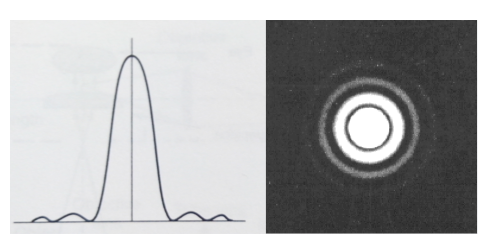
\includegraphics[width=0.7\textwidth]{capitulo2/airydisk}
\caption{Distribuci\'on de intensidad de un haz de luz y patr\'on de difracci\'on conocido como \emph{Airy Disk} \label{difra}}   %http://microscopy.berkeley.edu/courses/tlm/2P/index.html 
\end{figure}

A finales del siglo XIX el f\'isico Ernst Abbe, quien trabajaba en la fabrica de microscopios de Carl Zeiss demostr\'o que la potencia o alcance de la resoluci\'on espacial de un microscopio depende de la longitud de onda de la luz utilizada para formar la imagen y del \'angulo con que el objetivo colecta la luz o apertura angular; con esto Abbe defini\'o la  \emph{apertura num\'erica} del objetivo como:

\begin{equation}
NA= n sin(\Theta) \label{apnu}
\end{equation}

donde $\Theta$ es la mitad de la apertura angular del objetivo de microscopio y $n$ es el \'indice de refracci\'on del medio entre el objetivo y la muestra \cite{libro}. Entre m\'as grande sea el cono de luz que puede dirigirse a la lente m\'as grande ser\'a su apertura num\'erica. De la ecuaci\'on \ref{apnu} se puede ver que el m\'aximo valor que puede tomar la apertura num\'erica es el \'indice de refracci\'on; por lo que una manera de aumentar la apertura num\'erica es utilizar un medio de inmersi\'on con un \'indice de refracci\'on mayor que el aire, como puede ser el agua o aceite. N\'otese que el uso de objetivos de microscopio con apertura num\'erica grande, implica una disminuci\'on de la distancia entre la muestra y el objetivo. 

La resoluci\'on de un microscopio se define como la distancia $d$ entre dos part\'iculas adyacentes las cuales pueden ser percibidas como part\'iculas separadas. La resoluci\'on est\'a dada por el criterio Rayleigh:

\begin{equation}
d=\frac{1.22 \lambda}{2NA}
\end{equation}

donde $\lambda$ es la longitud de onda de la luz incidente en el vac\'io \cite{bioph}. De aqu\'i se  deduce que lentes con apertura \'optica mayor pueden brindar mejor resoluci\'on. 


El l\'imite de resoluci\'on por difracci\'on para un microscopio \'optico convencional, es decir, el detalle m\'as peque\~{n}o $\triangle x$ que puede ser resuelto con un microscopio en funci\'on de la longitud de onda $\lambda$ y apertura num\'erica $NA$ del objetivo es:

\begin{equation}
\triangle x=\frac{ \lambda}{2NA}
\end{equation}

Esta ecuaci\'on se conoce como la ecuaci\'on de Abbe \cite{libro}. La teor\'ia que desarrollo Abbe sobre el microscopio \'optico lo llevo a concluir que la resoluci\'on del microscopio est\'a determinada por la apertura num\'erica y no la magnificaci\'on; adem\'as concluy\'o que longitudes de onda m\'as cortas incrementan la resoluci\'on.

Otras distorsiones que se presentan en el sistema \'optico del microscopio e impiden la formaci\'on de una imagen perfecta se conocen como aberraciones. Hay dos tipos principales de aberraciones que desv\'ian la luz a causa de las propiedades de las lentes, o bien,  las formas geom\'etricas de las superficies reflejantes y de refracci\'on: aberraci\'on crom\'atica y esf\'erica. La primera se debe a la dependencia que tiene el \'inidce de refracci\'on con la longitud de onda, provocando que la luz se refracte con direcciones diferentes; mientras que la aberraci\'on esf\'erica se debe a la forma de las lentes, con distancias focales diferentes dependiendo de la zona de la lente.

El dise\~{n}o y manufactura de un microscopio buscan minimizar las aberraciones, maximizar la resoluci\'on y alcanzar la m\'axima fidelidad posible entre el objeto y la imagen con el contraste suficiente.  

El microscopio de fluorescencia ha emergido como una gran t\'ecnica para la adquisici\'on de im\'agenes de sistemas vivos; la fluorescencia proveniente de la muestra se utiliza para obtener la imagen. Se puede utilizar fluorescencia end\'ogena o se puede marcar el esp\'ecimen biol\'ogico con un fluor\'oforo, cuya distribuci\'on ser\'a evidente despu\'es de la iluminaci\'on. 

La microscopia de fluorescencia es idealmente utilizada para la detecci\'on de fluor\'oforos espec\'ificos en c\'elulas y tejidos. Se han desarrollado algunos microscopios cuyo funcionamiento se basa en la fluorescencia como el microscopio de epifluorescencia, confocal de barrido l\'aser y multifot\'on.


%%%%%%%%%% MICROSCOPIO DE epiFLUORESCENCIA %%%%%%%%%%%%%%%%%%%%%%%%%%%%%%%%%%%%  esp�cimen 

\subsection{Microscopio de epifluorescencia}


El microscopio m\'as utilizado hoy en d\'ia sigue el dise\~{n}o b\'asico de epifluorescencia. En este dispositivo la luz de excitaci\'on pasa a trav\'es del mismo objetivo de microscopio que posteriormente recolectar\'a la luz emitida por la muestra para formar la imagen; utilizando para ello filtros y un divisor de haz como se muestra en la figura \ref{epi}.

El divisor de haz transmite o refleja la luz dependiendo de su longitud de onda y separa la luz de excitaci\'on de la fluorescencia; la longitud de onda de la luz emitida es m\'as grande que la de excitaci\'on. En el sistema de iluminaci\'on se utilizan fuentes con un amplio rango espectral como l\'amparas de mercurio o xen\'on y con ayuda de un filtro se selecciona una longitud de onda espec\'ifica (com\'unmente en el rango UV). 

\begin{figure}[ht]
\centering
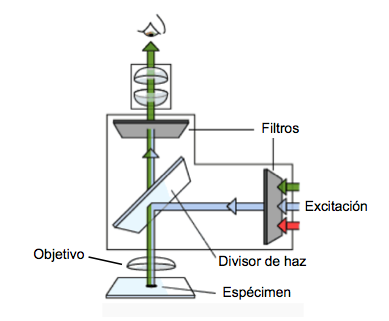
\includegraphics[width=3.2in, height=2.5in]{capitulo2/micrfluor}
\caption{Principio b\'asico de microscopio de epifluorescencia \label{epi}}    %http://www.nobelprize.org/educational/physics/microscopes/fluorescence/
\end{figure}

Este tipo de microscopio tiene varias ventajas: el objetivo (utilizado primero para concentrar y enfocar la luz incidente en la muestra y despu\'es como colector de la luz emitida para formar la imagen) siempre est\'a en correcta alineaci\'on; la mayor parte de la luz de excitaci\'on atraviesa el esp\'ecimen y se aleja del objetivo; la zona iluminada de la muestra se limita a lo que puede ser observado; se puede utilizar la apertura num\'erica completa del objetivo de microscopio; es posible combinar o alternar la manera de obtener la imagen, analizando la fluorescencia de la muestra o la luz transmitida \cite{ventajasepi}.


%%%%%%%%%%%%%%%%%%%%%%%%%%%%%%microscopia confocal de barrido laser
\subsection{Microscop\'ia confocal de barrido l\'aser}

La microscop\'ia confocal es una t\'ecnica que puede aumentar la resoluci\'on y el contraste de una imagen con el uso de una iluminaci\'on puntual y una abertura confocal en el camino del haz que forma la imagen (fluorescencia en el caso del microscopio de fluorescencia). El objetivo de la apertura, que puede ser un pinhole, es eliminar las contribuciones de la luz fuera de foco como se explica en el esquema de la figura \ref{confo}. 

\begin{figure}[ht]
\centering
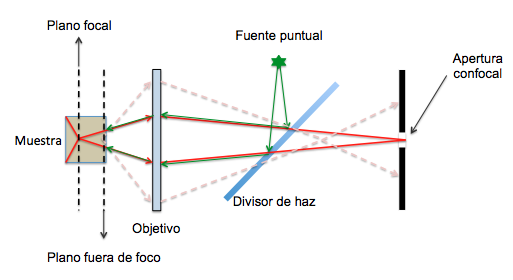
\includegraphics[width=0.95\textwidth]{capitulo2/confocal2}
\caption{\small{Trayectoria de la luz en un microscopio confocal de fluorescencia. La luz fuera del plano focal no es detectada debido a la apertura confocal.}\label{confo}}   
\end{figure}

La t\'ecnica que combina la microscop\'ia confocal y de fluorescencia es la microscop\'ia confocal de barrido l\'aser, en donde la fuente de excitaci\'on es un haz l\'aser enfocado por un objetivo a la muestra. La extensi\'on espacial del l\'aser enfocado en la muestra es determinado por la longitud de onda, la apertura num\'erica de las lentes y la calidad de formaci\'on de la imagen. 

La principal caracter\'istica de esta t\'ecnica es la capacidad de adquirir im\'agenes a profundidades espec\'ificas del tejido (de hasta 100 micrometros) permitiendo reconstrucciones en 3D. Otra ventaja de este dispositivo es que la magnificaci\'on puede ajustarse variando el \'area de barrido del l\'aser en la muestra sin necesidad de cambiar los objetivos, esta caracter\'istica se conoce como \emph{zoom factor} \cite{lscm}.

La fluorescencia utilizada para formar la imagen en este microscopio es inducida por la absorci\'on de un fot\'on y es un proceso lineal, por ello la fluorescencia se manifiesta a lo largo de un cono de luz como se observa en la imagen izquierda de la figura \ref{puntual}; esto puede provocar da\~{n}o fotoqu\'imico en un \'area grande de la muestra.

La mayor\'ia de fluor\'oforos utilizados en esta t\'ecnica, como marcadores en sistemas vivos son excitados por la absorci\'on de un fot\'on en la regi\'on UV o azul de la luz. A esta longitud de onda la luz es altamente atenuada por el tejido y limita la adquisici\'on de im\'agenes con gran profundidad de penetraci\'on \cite{bioph}.

\begin{figure}
\centering
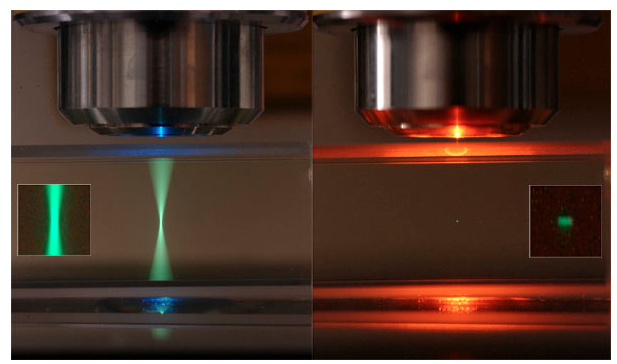
\includegraphics[width=0.7\textwidth]{capitulo2/compara}
\caption{Haz de excitaci\'on para microscop\'ia de barrido l\'aser de uno y dos fotones. \emph{\scriptsize{Imagen de  Steve Ruzin y Holly Aaron, UC Berkeley.}}\label{puntual}}   %http://microscopy.berkeley.edu/courses/
\end{figure}

%%%%%%%%%% MICROSCOPIO multifot�n %%%%%%%%%%%%%%%%%%%%%%%%%%%%%%%%%%%%  esp�cimen 
\subsection{Microscop\'ia multifot\'on}

En la microscop\'ia multifot\'on un fluor\'oforo es excitado mediante la absorci\'on de dos o mas fotones y la fluorescencia emitida se usa para formar una imagen. La fluorescencia inducida por la absorci\'on de dos o tres fotones se ha utilizado en este tipo de microscop\'ia no lineal. Sin embargo, por razones pr\'acticas (luz de excitaci\'on de gran intensidad) que requiere el proceso de absorci\'on de tres fotones, solo la microscop\'ia de dos fotones ha emergido como una de las t\'ecnicas m\'as utilizadas para adquisici\'on de im\'agenes de sistemas vivos. 

La absorci\'on de dos fotones es un fen\'omeno no lineal que fue propuesto te\'oricamente por Maria G\"{o}ppert- Mayer. En este proceso un \'atomo tiene una transici\'on del estado base $S_{0}$ al estado excitado $S_{n}$ por la absorci\'on "simult\'anea" de dos fotones (Ver Figura \ref{diagramatpa}); el primer fot\'on induce la trasici\'on del estado base a un estado virtual y el segundo fot\'on induce la transici\'on del estado virtual al estado excitado. 

\begin{figure}
\centering
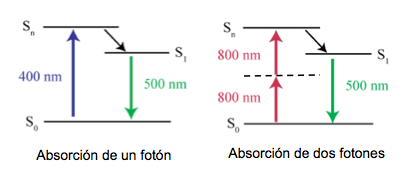
\includegraphics[width=4.2in, height=2.2in]{capitulo2/tpa1}
\caption{Diagrama de energ\'ia para la transici\'on de uno y dos fotones. \emph{\scriptsize{Imagen de D. Nowak}} 
 \label{diagramatpa}}    
\end{figure}

La probabilidad del proceso de absorci\'on de dos fotones depende de la intensidad de la luz de excitaci\'on elevada al cuadrado, por eso es necesario el uso de un l\'aser con pulsos intensos. La microscop\'ia de barrido l\'aser de dos fotones puede utilizar un l\'aser enfocado de pulsos cortos (del orden de picosegundos y femtosegundos) con longitud de onda en el rojo o cercano infrarrojo  como fuente de excitaci\'on y puede producir fluorescencia en el rango visible. 

El uso de un haz de excitaci\'on enfocado en esta t\'ecnica de microscop\'ia presenta ventajas como la implementaci\'on de resoluci\'on espacial sin el uso de \emph{pinholes}  o rendijas como filtros espaciales, la obtenci\'on de im\'agenes 3D y la confinaci\'on de la destrucci\'on fotoqu\'imica al volumen focal como se muestra en el lado derecho de la figura \ref{puntual}). Adem\'as como las c\'elulas y tejidos presentan relativa transparencia ante la radiaci\'on infrarroja (Ver Figura \ref{penetrad}), la microscop\'ia de barrido l\'aser de dos fotones aumenta la profundidad de penetraci\'on en espec\'imenes vivos; mientras m\'as grande sea la longitud de onda de la luz de excitaci\'on, el da\~{n}o a las c\'elulas y tejidos es menor.

Esta t\'ecnica es ideal para adquirir im\'agenes de diversas profundidades en tejidos, con una resoluci\'on de submicr\'ometros: $0.3\mu m$ de resoluci\'on lateral, $0.8\mu m$ de resoluci\'on axial y una profundidad de penetraci\'on que puede ir de $500$ a $1000\mu m$ \cite{libro}.

%En la pr\'actica la resoluci\'on espacial del microscopio de absorci\'on de dos fotones es similar al microscopio confocal de fluorescencia. El primero tiene una resoluci\'on ligeramente menor en comparaci\'on con el microscopio confocal pero el uso de una abertura confocal provoca p\'erdidas en la se\~{n}al.

\begin{figure}
\centering
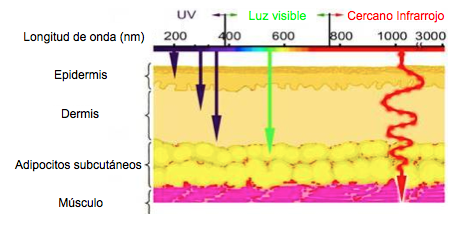
\includegraphics[width=4.5in, height=2.2in]{capitulo2/penetras}
\caption{Esquema de penetraci\'on del tejido a diferentes longitudes de onda \label{penetrad}}    
\end{figure}

\section{Propiedades \'opticas de marcadores en microscopia de fluorescencia}

Hay diversos materiales org\'anicos e inorg\'anicos que presentan una gran emisi\'on de luz y se utilizan como marcadores biocompatibles en microscop\'ia de fluorescencia. El estudio \'optico lineal y no lineal de estos materiales, desde colorantes comerciales hasta nanopart\'iculas de nuevos compuestos, incluye por ejemplo el an\'alisis de propiedades como la eficiencia cu\'antica de fluorescencia o la secci\'on transversal de absorci\'on de dos fotones, la cual es relevante para los marcadores en microscop\'ia de barrido l\'aser de dos fotones.

Por otra parte, un fen\'omeno que ha sido \'util en la microscop\'ia de fluorescencia, es la Transferencia de Energ\'ia de Resonancia F\"orster \'o FRET por sus siglas en ingl\'es. Esta transferencia de energ\'ia permite modificar algunas  propiedades \'opticas de un fluor\'oforo utilizando otro compuesto o colorante bajo ciertas condiciones mostradas m\'as adelante.  
  
\subsection{Eficiencia cu\'antica de fluorescencia}

Los procesos de decaimiento que llevan a una mol\'ecula  del estado excitado al estado base pueden ser radiativos y no radiativos. Como decaimientos no radiativos se pueden citar la conversi\'on interna y transiciones entre dos estados el\'ectronicos (que pueden llevar a la emisi\'on de fosforescencia) entre otros; sin embargo, el proceso de decaimiento predominante en el tipo de materiales que se estudiaron en este trabajo es radiativo: la fluorescencia; que es un tipo de luminiscencia con una tasa de emisi\'on de $10^{8} s^{-1}$ y un tiempo de vida de varios nanosegundos. 

%La luminiscencia puede ser fosforescencia o fluorescencia, dependiendo de la naturaleza del estado excitado. La tasa de emisi\'on de la fosforescencia es de $10^{3}$ a $1 s^{-1}$ y tiene un tiempo de vida del orden de milisegundos; sin embargo, la tasa de emisi\'on de la fluorescencia es t\'ipicamente del orden de  y tiene un tiempo de vida de varios nanosegundos .

La eficiencia cu\'antica de fluorescencia $\Phi_{f}$ es la raz\'on que hay entre los fotones absorbidos por un compuesto y los emitidos mediante fluorescencia como se muestra en la ecuaci\'on \ref{eficuan}. La eficiencia cu\'antica de fluorescencia, determina la probabilidad de que una mol\'ecula en estado excitado tenga un decaimiento radiativo por fluorescencia, en lugar de cualquier otro mecanismo no radiativo \cite{UK}.

\begin{equation}
\Phi_{f}=\frac{\# fotones \hspace{0.2cm} emitidos}{\# fotones  \hspace{0.2cm} absorbidos} \label{eficuan}
\end{equation}

Desde hace algunas d\'ecadas, se han realizado esfuerzos para desarrollar m\'etodos confiables que determinen la eficiencia cu\'antica de fluorescencia, la mayor\'ia de los cuales utilizan el compuesto de inter\'es en soluci\'on o suspensi\'on.

Los m\'etodos que buscan determinar directamente la eficiencia cu\'antica de fluorescencia, se conocen como m\'etodos absolutos. Por ejemplo el m\'etodo Vavilov, monitorea la fluorescencia de la muestra en una celda y el esparcimiento de una superficie s\'olida de \'oxido de magnesio; en el m\'etodo de Weber y Teale, a diferencia del anterior, se analiza el esparcimiento de una soluci\'on y el m\'etodo calor\'imetrico, mide la energ\'ia liberada en forma de calor por los decaimientos no radiativos. 

Debido a las complejas correcciones que requieren diversos m\'etodos absolutos, en la gran mayor\'ia de laboratorios se utiliza el m\'etodo relativo para medir $\Phi_{f}$. Este m\'etodo se basa en comparar la intensidad de fluorescencia de la muestra de inter\'es con la intensidad de fluorescencia de una soluci\'on de referencia \cite{tesisdoc}. En particular, en este trabajo se midi\'o la eficiencia cu\'antica de fluorescencia con un m\'etodo relativo utilizando una esfera integradora.

\subsubsection{M\'etodo relativo de la esfera integradora para medir eficiencia cu\'antica de fluorescencia}

En este m\'etodo se mide la eficiencia cu\'antica de fluorescencia $ \Phi_f$ para un compuesto en soluci\'on o suspensi\'on de nanopart\'iculas mediante la detecci\'on de emisi\'on de luz de \'este en una esfera integradora; para ello se utiliza un sistema de detecci\'on, que puede ser constituido por un monocromador, una c\'amara CCD, un analizador multicanal fot\'onico, un fotodetector etc... Particularmente, en este trabajo se utiliz\'o un un tubo fotomultiplicador o PMT por sus siglas en ingles y un amplificador lock- in. 

Las soluciones o suspensiones se colocan en celdas de cuarzo de $0.1\times1\times4 cm^{3}$ a concentraciones del orden de $10^{-6}$ y $10^{-7}$ M. La emisi\'on de luz de la muestra es reflejada con la misma intensidad en todas direcciones dentro de la esfera integradora y detectada por un PMT colocado en una abertura de la esfera. El PMT, detecta los fotones de emisi\'on y crea una se\~{n}al el\'ectrica que es enviada a un amplificador lock- in. Finalmente el amplificador arroja el valor, en volts, de la se\~{n}al causada por la intensidad de fluorescencia.

El proceso anterior se repite para una soluci\'on utilizada como referencia con valor de eficiencia cu\'antica de fluorescencia conocido. Comparando la emisi\'on de luz de la muestra de inter\'es con la emisi\'on de luz de la referencia se puede conocer $\Phi_f$ para la muestra, como se explica a continuaci\'on. 

Cuando el haz de excitaci\'on incide en un medio, en este caso la celda, parte de la luz ser\'a transmitida, reflejada y absorbida por el medio. La aplicaci\'on de la conservaci\'on de energ\'ia, determina que la suma de la transmisi\'on $t$ , reflexi\'on $r$ y absorci\'on $a$ de la luz incidente es igual a la unidad.

\begin{equation}
t+r+a=1  \label{1}
\end{equation}  

En el m\'etodo utilizado en este trabajo, el reflejo del haz de excitaci\'on en la celda se dirigi\'o hacia afuera de la esfera integradora para no ser detectado y as\'i suponer que $r=0$ en la ecuaci\'on \ref{1}. %%%no es cierto en la realidad la luz reflejada es distinta de cero pero su contribuci�n se elimina utilizando tambi�n la referencia!!!!

La intensidad de la luz emitida por una muestra $I_m$ es proporcional a la intensidad de luz del haz incidente $I_{0 _m}$, eficiencia cu\'antica de fluorescencia $\Phi_{f_m}$ y absorci\'on $a$; esta \'ultima se puede expresar como $a=1-t$ para escribir:

\begin{equation}
I_{m}\propto I_{0m} \Phi_{f_m}(1-t) \label{prop}
\end{equation}  

N\'otese que se ha utilizado el sub\'indice $m$ para hacer referencia a los par\'ametros de la muestra de inter\'es. Utilizando la Ley de Lambert- Beer es posible expresar la transmisi\'on como $t=10^{-A_{m}}$, donde $A_{m}$ es la absorbancia de la muestra. La ecuaci\'on \ref{prop} puede escribirse como 

\begin{equation}
I_{m}=k I_{0m} \Phi_{m}(1-10^{-A_{m}}) \label{igual}
\end{equation}  
 
donde se introdujo la constante instrumental $k$. El valor de esta constante de correcci\'on para el sistema completo de medici\'on de eficiencia cu\'antica no es conocido, pero puede ser eliminado de la ecuaci\'on \ref{igual} utilizando una soluci\'on de prueba o referencia con valor de eficiencia cu\'antica de fluorescencia conocido. Es decir, la intensidad de emisi\'on de la muestra de referencia $I_{ref}$ es  $I_{ref}=k I_{0 ref} \Phi_{f_{ref}}(1-10^{-A_{ref}})$, donde se especifica que se trata de la referencia con el sub\'indice $ref$. 

En los experimentos realizados en este trabajo, se midi\'o la intensidad de fluorescencia de la muestra de inter\'es y de la referencia bajo las mismas condiciones y se utiliz\'o la misma intensidad de excitaci\'on\footnote{No es una condici\'on necesaria cuando el sistema de detecci\'on responde de manera lineal para distintos valores de intensidades incidentes de inter\'es}, es decir, $I_{0m}=I_{0 ref}$. Bajo estas circunstancias, resolviendo el sistema de ecuaciones para $\Phi_{f_m}$ se tiene que: 

\begin{equation}
\Phi_{f_m}= \Phi_{f_{ref}} \frac{I_{m}}{I_{ref}} \frac{(1-10^{-A_{ref}})}{(1-10^{-A_{m}})}  \label{final}
\end{equation}  
 
$ \Phi_{f_{ref}}$ es el valor conocido de la eficiencia cu\'antica de fluorescencia para la referencia. En este experimento $I_{m}$ e $I_{ref}$ son par\'ametros referentes a la detecci\'on del nivel de intensidad de emisi\'on de la muestra y de la referencia, cuyos valores (al ser detectados con un PMT) est\'an dados en volts; los valores de absorbancia para la muestra y la referencia a la misma longitud de onda que el haz de excitaci\'on se conocen con los espectros de absorci\'on, los cuales se adquieren en celdas de cuarzo con la misma longitud de camino \'optico y la misma concentraci\'on molar que se utilizaron en este m\'etodo.
 
  
%Essentially, solutions of the standard and test samples with identical absorbance at the same excitation wavelength can be assumed to be absorbing the same number of photons.

\subsection{Procesos no lineales: Absorci\'on de dos fotones}

La \'optica no lineal estudia los fen\'omenos que ocurren como consecuencia de la modificaci\'on de las propiedades \'opticas de un material por la presencia de luz, t\'ipicamente luz l\'aser. Los fen\'omenos \'opticos son no lineales, porque ocurren cuando la respuesta de un material al campo \'optico aplicado depende de una manera no lineal de la amplitud de dicho campo \'optico \cite{boyd}.

Para comprender lo anterior es importante analizar la dependencia que tiene la polarizaci\'on de un material con la amplitud del campo el\'ectrico aplicado. En la \'optica convencional o lineal, la polarizaci\'on inducida depende linealmente de la amplitud del campo el\'ectrico; sin embargo, en \'optica no lineal la respuesta se generaliza expresando la polarizaci\'on inducida $P(t)$ como sigue:
 
\begin{equation}
\label{que}
P(t)=\epsilon_{0}[\chi^{(1)}E(t)+\chi^{(2)} E^2(t)+\chi^{(3)} E^{3}(t)+...]
\end{equation}

donde $\epsilon_{0}$ es la permitividad en el vac\'io y $\chi^{(1)}$, $\chi^{(2)}$ y  $\chi^{(3)}$ representan la susceptibilidad el\'ectrica de primero, segundo y tercer orden respectivamente. Por simplicidad, en la ecuaci\'on anterior \'unicamente se toma en cuenta el car\'acter escalar tanto de la polarizaci\'on como del campo el\'ectrico y se asume una polarizaci\'on instant\'anea y por lo tanto una susceptibilidad el\'ectrica constante (no hay p\'erdidas ni dispersi\'on). 

La polarizaci\'on juega un papel importante en la descripci\'on de fen\'omenos no lineales porque cuando var\'ia en el tiempo, puede actuar como fuente de nuevos componentes del campo electromagn\'etico.

La absorci\'on de dos fotones es una consecuencia de la polarizaci\'on no lineal de tercer orden, dicha polarizaci\'on se puede identificar de la ecuaci\'on \ref{que} como $P^{(3)}(t)=\epsilon_{0}\chi^{(3)} E^{3}(t)$. Si se considera un campo el\'ectrico monocrom\'atico de la forma $E(t)=\xi cos(wt)$, incidiendo en un material tal que $\chi^{(3)}\neq0$ \footnote{La susceptibilidad el\'ectrica de tercer orden es diferente de cero sin importar el material, puede ser un medio centrosim\'etrico o no centrosim\'etrico.}, la polarizaci\'on no lineal de tercer orden se expresa como:

\begin{equation}
\label{que2}
P^{(3)}(t)=\frac{1}{4}\epsilon_{0}\chi^{(3)}\xi^{3} cos(3wt)+\frac{3}{4}\epsilon_{0}\chi^{(3)}\xi^{3} cos(wt) 
\end{equation}

donde se utiliz\'o la identidad trigonom\'etrica $cos^{3}(w)= \frac{1}{4} cos(3wt)+\frac{3}{4} cos(wt)$. El primer t\'ermino de la ecuaci\'on \ref{que2} describe una respuesta de frecuencia $3w$ creada por un campo incidente de frecuencia $w$, este proceso se conoce como generaci\'on de tercer arm\'onico o THG por sus siglas en ingl\'es. 

El segundo t\'ermino de la ecuaci\'on \ref{que2} describe la contribuci\'on no lineal de la polarizaci\'on a la misma frecuencia que el campo incidente; este t\'ermino, como se explica m\'as adelante, es la contribuci\'on no lineal al \'indice de refracci\'on que experimenta una onda de frecuencia $w$. En la figura \ref{dibujo3o} se muestra un medio no lineal en el que incide un campo de frecuencia $w$, la polarizaci\'on no lineal de tercer orden creada en este medio tiene contribuciones de frecuencias $w$ y $3w$.

\begin{figure}[ht]
\centering
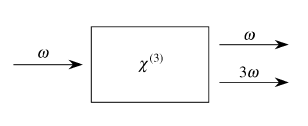
\includegraphics[width=0.6\textwidth]{capitulo2/tercerorden}
\caption{Geometr\'ia del efecto de la polarizaci\'on no lineal de tercer orden \label{dibujo3o}}   
\end{figure}

De manera general, el estudio de la polarizaci\'on no lineal de tercer orden se desarrolla considerando un campo el\'ectrico incidente compuesto por  tres frecuencias no necesariamente iguales, por lo que habr\'a diversas  contribuciones a la polarizaci\'on no lineal correspondientes a las frecuencias resultantes de la combinaci\'on de las frecuencias incidentes (Generaci\'on de terceros arm\'onicos, diferencia y suma de frecuencias y las mismas frecuencias incidentes).  

Para visualizar lo anterior, consid\'erese un campo el\'ectrico polarizado en la direcci\'on $i$ incidiendo en un material no lineal; si se toma en cuenta que la polarizaci\'on no es instant\'anea, la polzarizaci\'on no lineal de tercer orden en el dominio de la frecuencia se escribe como:
 
\begin{equation}
P_i^{(3)}(\vec{r},w_4)=\triangle \epsilon_0 \chi^{(3)}_{ijkl}(-w_4;w_1,w_2,w_3)E_j(\vec{r},w_1)E_k(\vec{r},w_2) E_l(\vec{r},w_3) \label{wt}
\end{equation}   

donde $ \chi^{(3)}_{ijkl}$ es el tensor de susceptibilidad de tercer orden\footnote{N\'otese que el tensor de susceptibilidad el\'ectrica de tercer orden es un tensor de cuarto grado (En tres dimensiones tiene 81 componentes)} y se cumple la relaci\'on $w_4=w_1+w_2+w_3$.  El s\'imbolo $\triangle$ toma los valores de $1$ cuando $w_1=w_2=w_3$, $\triangle = 3$ cuando dos de las frecuencias son iguales y $\triangle=6$ si todas las frecuencias son diferentes.

Si se considera un campo incidente de frecuencia $w$ y se analiza la contribuci\'on a la polarizaci\'on no lineal de tercer orden correspondiente a la misma frecuencia incidente $w$, la ecuaci\'on \ref{wt} se expresa de la siguiente manera:

\begin{equation}
P_i^{(3)}(\vec{r},w)=3  \epsilon_0 \chi^{(3)}_{ijkl}(-w;w,w,-w)E_j(\vec{r},w)E_k(\vec{r},w) E^{\ast}_l(\vec{r},w)
\end{equation}

donde $E^{\ast}_l(\vec{r},w)=E_l(\vec{r},-w)$. Si el material es isotr\'opico, es decir, sus propiedades son las mismas en todas direcciones y asumimos que $i=j=k$, entonces debe observarse que $i=j=k=l$ y la expresi\'on anterior se escribe como $P^{(3)}(\vec{r},w)=3  \epsilon_0 \chi^{(3)}(-w;w,w,-w)E(\vec{r},w) |E (\vec{r},w)|^2$. As\'i la polarizaci\'on total $P_T(\vec{r},w)$ para este caso en el que hay un campo incidente de frecuencia $w$ se escribe como:

\begin{align}
P_T(\vec{r},w)=\epsilon_0[ \chi^{(1)}+ 3 \chi^{(3)} |E(\vec{r},w)|^2] E(\vec{r},w)\label{pt} 
\end{align}

La polarizaci\'on de segundo orden es cero porque $\chi^{(2)} \neq 0$ \'unicamente en medios no centrosim\'etricos.

Por otro lado, la ecuaci\'on de onda en el dominio de la frecuencia $\Omega$ se expresa como $\nabla^2\vec{E}(\vec{r},\Omega)+\frac{\Omega^2}{c^2}\vec{E}(\vec{r},\Omega)=-\mu_{0}\Omega^2\vec{P}(\vec{r},\Omega)$,donde $\mu_{0}=\frac{1}{c^{2} \epsilon_{0}}$ es la constate magn\'etica en el vac\'io.

Si en la polarizaci\'on total de la ecuaci\'on \ref{pt} se considera un campo el\'ectrico polarizado en direcci\'on $i$, cuya direcci\'on de propagaci\'on est\'a en la direcci\'on $z$ ($\vec{r}=z\hat{k}$), entonces la ecuaci\'on de onda en el dominio de la frecuencia se escribe como:

\begin{align}
\frac{\partial^2}{\partial z^2}E_{i}(z,w)+\left[\frac{w}{c}\right]^2 E_{i}(z,w)=-\frac{w^2}{c^2}[\chi^{(1)}_{ii}E_{i}(z,w)+\chi^{(3)}_{iiii}|E(z,w)|^2 E_{i}(z,w)]
\end{align}
 
Proponiendo la soluci\'on $E_{i}(z,w)=\xi(z)e^{ikz}$ y utilizando la Aproximaci\'on de Envolvente de Variaci\'on Lenta\footnote{En esta aproximaci\'on la amplitud $\xi(z)$ varia muy lentamente por lo que $\frac{d\xi_{i}(z)}{dz}\gg \frac{d^2\xi_{i}(z)}{dz^2}$} (SVEA) se tiene que:

\begin{align}
\frac{d\xi(z)}{\xi(z)}=\frac{3i}{2k}\left[\frac{w}{c}\right]^2 \chi^{(3)}_{iiii} |\xi(z)|^2 dz\label{svea}
\end{align}

en donde $(1+\chi^{(1)}_{ii})(w^2/c^2)=k^2$. 

Si se asume que que $\chi^{(3)}_{iiii}$ es real y se integra la ecuaci\'on \ref{svea} se obtiene como soluci\'on $E(z,w)=\xi_0 e^{i\{ \frac{w}{c}n+  \frac{3}{2}\frac{w}{c}\frac{1}{n} \chi^{(3)}_{iiii} |\xi_0|^2\}z}$ donde se utiliz\'o que $k=\frac{w}{c}n$. En analog\'ia con el r\'egimen lineal se puede apreciar que el \'indice de refracci\'on total $n_T$ , ahora tiene la contribuci\'on no lineal  $\frac{3}{2}\frac{1}{n} \chi^{(3)}_{iiii} |\xi_0|^2$; por lo que en t\'erminos de intensidad se tiene que el \'indice de refracci\'on total $n_T$ es:

\begin{align}
n_T=n+  n_2 I
\end{align}

donde $n_2=\frac{3\chi^{(3)}_{iiii}}{\epsilon_0 n^2c}$ es el \'indice de refracci\'on no lineal de intensidad conocido como coeficiente Kerr y la intensidad es $I=\frac{1}{2}n\epsilon_0 c  |\xi(z)|^2$. %Esto indica que en el r\'egimen no lineal el \'indice de refracci\'on depende de la intensidad.

Sin embargo, el tensor de susceptibilidad el\'ectrica de tercer orden tiene tambi\'en una parte imaginaria. Para conocer el efecto de absorci\'on se asume ahora que $\chi^{(3)}_{real}=0$, por lo que sustituyendo $\chi^{(3)}=i \chi^{(3)}_{im}$ en la ecuaci\'on \ref{svea} se obtiene $\frac{d|\xi(z)|^2}{dz}=-\beta_E|\xi(z)|^4$, donde se ha definido $\beta_E=\frac{3w\chi^{(3)}_{im}}{cn}$ como el coeficiente de absorci\'on no lineal referente al capo el\'ectrico. Y en t\'erminos de la intensidad: 

\begin{align}
\frac{dI}{dz}=-\beta I^2 \label{porfin}
\end{align}

donde $\beta=\frac{6w\chi^{(3)}_{im}}{c^2n_f^2 \epsilon_0}$ es el coeficiente de absorci\'on no lineal referente a la intensidad. As\'i, tanto el coeficiente de refracci\'on $n_2$ como el coeficiente de absorci\'on $\beta$ no lineales dependen de la intensidad.

Tomando en cuenta la absorci\'on lineal mediante la Ley de Lambert- Beer la ecuaci\'on \ref{porfin} se escribe como:

\begin{align}
\frac{dI}{dz}=-\alpha I  -\beta I^2=-\alpha_T I
\end{align}

donde $\alpha$ es el coeficiente de absorci\'on lineal y $\alpha_T (I)=\alpha+\beta I$ es el coeficiente de absorci\'on efectivo del material. La soluci\'on de esta ecuaci\'on diferencial es: $I(z)=\frac{\alpha e^{-\alpha z}}{1-\beta e^{-\alpha z}}$, lo cual da lugar a dos tipos de absorci\'on dependiendo del signo de $\beta$.  

Si $\beta<0$ el coeficiente de absorci\'on efectivo disminuye cuando la intensidad crece, esto se conoce como absorci\'on saturable. Esta absorci\'on vuelve a los materiales transparentes a medida que la intensidad del campo el\'ectrico incidente aumenta.


Sin embargo, cuando $\beta>0$ el coeficiente de absorci\'on efectivo aumenta con la intensidad como se muestra en la figura \ref{grafiquita}. Este proceso se conoce como absorci\'on de dos fotones; fue descrito por primera vez, de forma te\'orica por Maria Goppert- Mayer en 1931 \cite{megalibro} y observado experimentalmente por Kaiser y Garret en 1961 \cite{boyd}.

\begin{figure}[ht]
\centering
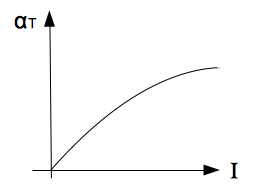
\includegraphics[width=0.34\textwidth]{capitulo2/gra2}
\caption{Absorci\'on de dos fotones \label{grafiquita}}   
\end{figure}

En este proceso, un \'atomo hace una transici\'on del estado base a un estado excitado mediante la absorci\'on \emph{simult\'anea} de dos fotones como se muestra en la figura \ref{diagramatpa}. Se dice que este proceso es simult\'aneo porque dos fotones deben interactuar en un estado virtual en un tiempo $\tau$ de $10^{-15}$ o $10^{-16}s$ para que se de la absorci\'on y el \'atomo sea promovido al estado excitado \cite{todoTPA}. La probabilidad de absorci\'on de dos fotones es proporcional al cuadrado de la intensidad de excitaci\'on. 

%Una aplicaci\'on basada en los efectos de la absorci\'on de dos fotones es un limitador \'optico que no permite el paso de luz si la intensidad es grande, evitando as\'i posibles da\~{n}os en circuitos \'opticos.


El efecto de absorci\'on de dos fotones se puede cuantificar introduciendo un par\'ametro conocido como secci\'on transversal de absorci\'on de dos fotones $\sigma^{TPA}$, el cual determina la magnitud del mismo proceso de absorci\'on. 

De la misma manera que la secci\'on transversal de absorci\'on lineal est\'a relacionada con el coeficiente de absorci\'on lineal, la relaci\'on entre $\beta$ y $\sigma^{TPA}$ es:

\begin{align}
\beta=N_g \frac{\sigma^{TPA}}{\hbar w}
\end{align}

donde $N_g$ es el n\'umero de mol\'eculas por volumen en el estado base. As\'i la ecuaci\'on \ref{porfin} se puede escribir de la siguiente manera:

\begin{align}
\frac{dI}{dz}= -N_g \sigma^{*TPA} I^2= -N_g \frac{\sigma^{TPA}}{\hbar w} I^2
\end{align}

donde $\sigma^{*TPA}$ es un coeficiente relacionado con la absorci\'on de dos fotones \cite{rescatetpa}. Las unidades de la secci\'on transversal de absorci\'on de dos fotones $\sigma^{TPA}$ son los G\"oppert- Mayer o [GM] (1GM=$10^{-50} cm^4 s fot\'on^{-1} mol\'ecula^{-1}$) mientras que las unidades de $\sigma^{*TPA}$ son [$longitud^4  mol\'ecula^{-1} potencia^{-1}$].

En t\'erminos del flujo de fotones $f$ teniendo en cuenta que $f=I/\hbar w$ la ecuaci\'on anterior se expresa como: $\frac{df}{dz}= -N_g \sigma^{TPA} f^2 \label{flujo}$. Sin embargo, el t\'ermino $df/dz$ representa la velocidad de atenuaci\'on por la absorci\'on de dos fotones a lo largo de la direcci\'on de propagaci\'on; esto significa que el n\'umero de fotones absorbidos $N(t)$ por unidad de tiempo y volumen es:
 
\begin{align}
N(t)= -\frac{df}{dz}=N_g \frac{\sigma^{TPA}}{(\hbar w)^2} I^2=\frac{\beta I^2}{\hbar w}
\end{align}


Hay diversas t\'ecnicas experimentales para determinar $\sigma^{TPA}$ o bien $\beta$, pueden ser t\'ecnicas directas, indirectas y de mezcla de ondas.

Los m\'etodos directos se basan en medir la atenuaci\'on de un haz l\'aser al atravesar el medio absorbedor; en los m\'etodos indirectos se mide uno de los efectos inducidos por la absorci\'on de dos fotones y en el mezclado de ondas se utiliza m\'as de un haz, com\'unmente incidiendo en direcciones diferentes en el medio.


\subsection{Medici\'on de $\sigma^{TPA}$ mediante la t\'ecnica de TPEF}

Un material que presenta una absorci\'on de dos fotones pasa del estado base al estado electr\'onico excitado. Despu\'es de un relajamiento inicial no radiativo, la energ\'ia de excitaci\'on restante se libera mediante uno o m\'as procesos f\'isicos; los m\'etodos indirectos que determinan $\sigma^{TPA}$ monitorean uno de los posibles procesos de de- excitaci\'on que llevan al \'atomo al estado base.

La t\'ecnica indirecta m\'as com\'un, utilizada en este trabajo, se denomina t\'ecnica de emisi\'on inducida por absorci\'on de dos fotones (TPEF por sus siglas en ingl\'es). En esta t\'ecnica se utiliza un haz l\'aser de gran intensidad, generalmente pulsado y enfocado para concentrar la energ\'ia en la muestra, y se mide la se\~{n}al de fluorescencia generada por la absorci\'on de dos fotones; de esta se\~{n}al de fluorescencia se puede determinar la secci\'on transversal de excitaci\'on de dos fotones $\sigma^{TPE}$, la cual es linealmente proporcional a la secci\'on transversal de absorci\'on de dos fotones $\sigma^{TPA}$ \cite{pre_rigo}, o bien:

\begin{align}
\sigma^{TPE}=\Phi_f \sigma^{TPA}
\end{align}

Como se vio en la secci\'on anterior el n\'umero de fotones absorbidos $N(t)$ por mol\'ecula, por unidad de tiempo es proporcional a la secci\'on transversal de absorci\'on de dos fotones y del cuadrado de la intensidad incidente. Sin embargo en un experimento particular, el n\'umero total de fotones absorbidos $N_{abs}(t)$ est\'a en funci\'on tambi\'en de la concentraci\'on $c$ de la muestra y del volumen $V$ iluminado en la misma \cite{maso}:

\begin{align}
N_{abs}(t)=\int_V \sigma^{TPA} c I^2(\vec{r},t)dV
\end{align}

Adem\'as se suele separar la dependencia temporal y espacial de la intensidad de excitaci\'on, es decir, $I^2(\vec{r},t)=S(\vec{r})I_0(t)$. Por lo que lo anterior se escribe como:

\begin{align}
 N_{abs}(t)= \sigma^{TPA} c I_0^2(t)\int_V  S^2(\vec{r})dV \label{k}
\end{align}

Por otra parte, el n\'umero total de fotones absorbidos por unidad de tiempo $N_{abs}(t)$ en un proceso de absorci\'on de dos fotones, est\'a relacionado con el n\'umero de fotones de fluorescencia $F(t)$ detectados en el experimento de la siguiente manera: $F(t)=\frac{1}{2}\eta \Phi_f N_{abs}(t)$, donde $\eta$ es la eficiencia de colecci\'on de fluorescencia del sistema experimental. N\'otese que el factor de $1/2$ refleja el hecho de que dos fotones son necesarios en cada evento de excitaci\'on.

Sin embargo, en la pr\'actica solo el promedio temporal del flujo de fotones emitidos $\langle F(t)\rangle$ es medido, es decir: 

\begin{align}
\langle F(t)\rangle=\frac{1}{2} \eta \Phi_f c \sigma^{TPA} \langle I_0^2(t)\rangle \int_V dV S^2(\vec{r})
\end{align}

donde se utiliz\'o el valor de $N_{abs}(t)$ de la ecuaci\'on \ref{k}. Como la mayor\'ia de los detectores entregan solo la se\~{n}al proporcional a $\langle I_0(t)\rangle$ se introduce el par\'ametro $g=\langle I_0^2(t)\rangle/\langle I_0(t)\rangle^2$ o grado de coherencia temporal de segundo orden\footnote{El grado de coherencia temporal de segundo orden se refiere a las fluctuaciones temporales del flujo de fotones incidentes}, de tal manera que la ecuaci\'on anterior se escribe como.

\begin{align}
\langle F(t)\rangle= \frac{1}{2} g \eta \Phi_f c \sigma^{TPA} \langle I_0(t)\rangle^2 \int_V dV S^2(\vec{r})  \label{yacasi}
\end{align}

De lo anterior es posible notar que la determinaci\'on experimental de $\sigma^{TPA}$ implica la caracterizaci\'on de cuatro par\'ametros: la disribuci\'on espacial de la luz incidente, el grado de coherencia temporal de segundo orden $g$, la eficiencia de colecci\'on de luz $\eta$ y la eficiencia cu\'antica de fluorescencia de la muestra $\Phi_f$ \cite{maso}.

La dependencia espacial de la ecuaci\'on \ref{yacasi} se resuelve considerando una distribuci\'on de intensidad en el volumen focal limitado por la difracci\'on de una apertura, en este caso una lente; definiendo las intensidades de los pulsos como intensidades instant\'aneas promediadas con respecto a la duraci\'on del pulso y utilizando m\'etodos num\'ericos para encontrar la soluci\'on de la integral. Para la dependencia temporal se considera un l\'aser pulsado como haz de excitaci\'on siendo $I_0(t)$ una funci\'on peri\'odica en el tiempo; se considera una excitaci\'on pulsada porque en este trabajo se determin\'o experimentalmente $\sigma^{TPA}$ utilizando un l\'aser de femtosegundos.

Por la naturaleza peri\'odica del tren de pulsos es necesario calcular $g$ solo para un ciclo, para eso se introduce la cantidad adimensional $g_p$ que cumple la relaci\'on $g=g_p/(f \tau)$; donde $f$ es la frecuencia de repetici\'on del haz y $\tau$ es el ancho temporal a media altura del pulso o FWHM por sus siglas en ingl\'es \cite{maso}. Asumiendo entonces una fuente de excitaci\'on pulsada, el promedio temporal de la fluorescencia detectada se puede escribir como:

\begin{align}
\langle F(t)\rangle \approx  \frac{1}{2}  \eta \Phi_f c \sigma^{TPA} \frac{g_p}{f \tau}     \frac{8n\langle P(t)\rangle^2}{\pi \lambda}     
\end{align}

donde $n$ es el indice de refracci\'on, $\langle P(t)\rangle$ es el promedio temporal de la potencia incidente y $\lambda$ es la longitud de onda del haz de excitaci\'on.

La fluorescencia depende fuertemente de la coherencia temporal del pulso de excitaci\'on, por lo que la determinaci\'on precisa de $\sigma^{TPA}$ requiere el conocimiento de $g$ en la regi\'on focal, lo cual no es trivial \cite{refderef}. Sin embargo en el m\'etodo descrito por Albota, Xu y Webb \cite{pre_rigo}, utilizado en este trabajo, las complicaciones de medir $g$ dentro de la muestra se evitaron utilizando una muestra de referencia con valor conocido de secci\'on transversal de absorci\'on de dos fotones.  Por lo que la raz\'on entre la se\~{n}al de fluorescencia de la muestra de referencia $\langle F(t)\rangle_{ref}$  y la muestra de inter\'es $\langle F(t)\rangle$ determinar\'a $\sigma^{TPA}$ para la nueva muestra:


\begin{align}
\frac{\langle F(t)\rangle_{ref} }{\langle F(t)\rangle } =  \frac{\eta_{ref} \Phi_{f_{ref}} c_{ref} \sigma^{TPA}_{ref} \langle P(t)\rangle_{ref}^2 n_{ref}}{\eta \Phi_f c \sigma^{TPA} \langle P(t)\rangle^2 n}  
\end{align}

donde los sub\'indices $ref$ indican los par\'ametros de la muestra de referencia mientras que los par\'ametros sin sub\'indice pertenecen a la muestra de inter\'es. Despejando $\sigma^{TPA}$ de la igualdad anterior se obtiene finalmente:

\begin{align}
 \sigma^{TPA}=  \frac{\eta_{ref} \Phi_{f_{ref}} c_{ref} \sigma^{TPA}_{ref} \langle P(t)\rangle_{ref}^2 n_{ref} \langle F(t)\rangle   }{\eta \Phi_f c \langle P(t)\rangle^2 n    \langle F(t)\rangle_{ref} }\label{finalsigma}  
\end{align}



\subsection{Transferencia de Energ\'ia de Resonancia F\"orster (FRET)\label{fretis}}

En esta modalidad, la energ\'ia es transferida mediante un proceso no radiativo entre una mol\'ecula donadora y una mol\'ecula aceptora en resonancia. La mol\'ecula donadora es excitada por un haz de luz y la energ\'ia de excitaci\'on es transferida a la mol\'ecula aceptora; simult\'aneamente la mol\'ecula donadora vuelve a su estado base. El mecanismo de esta transferencia de energ\'ia de resonancia involucra interacciones d\'ebiles de tipo diolo--dipolo, las cuales se dan cuando la distancia entre la mol\'ecula donadora y aceptora es mucho mayor que sus dimensiones.

Para dos mol\'eculas poliat\'omicas en soluci\'on, una mol\'ecula donadora y otra aceptora, el espectro de absorci\'on de la mol\'ecula aceptora debe traslaparse con el espectro de emisi\'on de la mol\'ecula donadora (Ver Figura \ref{fretito}).

\begin{figure}[ht]
\centering
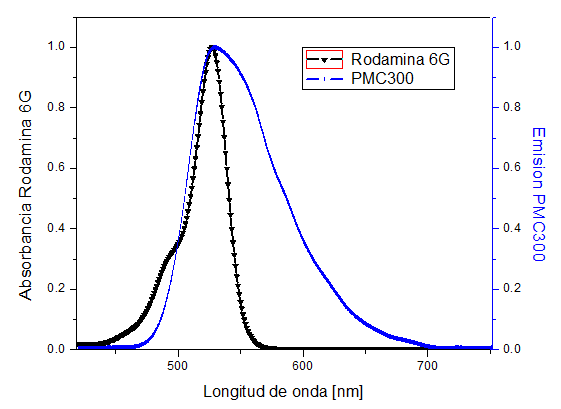
\includegraphics[width=0.5\textwidth]{capitulo2/fret}
\caption{\small{Esquema de la Transferencia de Energ\'ia de Resonancia F\"orster}\label{fretito}}   
\end{figure}

Los antecedentes de la t\'ecnica FRET comenzaron en 1922 con el trabajo experimental de Cario sobre lo que denomin\'o \emph{fluorescencia sensibilizada}. Cario introdujo vapor de mercurio y talio en un tubo de cuarzo, lo ilumin\'o utilizando una l\'ampara de mercurio a 253.5$nm$ y lo que observ\'o fue la emisi\'on de los \'atomos de talio;  en ausencia del mercurio, los \'atomos de talio no fueron excitados a dicha longitud de onda. %La transferencia de enrg\'ia fue explicada mediante colisiones de los \'atomos de ambos elementos.

Las primeras observaciones de fluorescencia sensibilizada en soluci\'on fueron realizadas por Jean Perrin y C. R. Choucroun en 1929. J. Perrin explic\'o la transferencia de energ\'ia por resonancia utilizando f\'isica cl\'asica y realiz\'o experimentos para analizar la polarizaci\'on de luz emitida por mol\'eculas en soluci\'on en funci\'on de la concentraci\'on. %A medida que la concentraci\'on aumentaba, la distancia promedio entre las mol\'eculas disminu\'ia, y por el aumento de probabilidad de transferencia de energ\'ia de excitaci\'on no radiativa, la polarizaci\'on medida se reduc\'ia.

En 1929 Kallmann y London presentaron una teor\'ia para explicar la transferencia de energ\'ia de resonancia desde el punto de vista de la mec\'anica cu\'antica. Esta teor\'ia consider\'o una interacci\'on de tipo dipolo--dipolo e introdujo el par\'ametro $R_0$ para referirse a la distancia entre el sistema donador y aceptor en la cual, la transferencia de energ\'ia y el decaimiento radiativo del sistema donador en estado excitado son igualmente probables. Kallmann y London calcularon que la probabilidad $P$ de que se presente una transferencia de energ\'ia es $P\propto \frac{1}{1+(\frac{R}{R_0})^6}$, donde $R$ es la distancia de separaci\'on que hay entre los dos sistemas en que se da la transferencia de energ\'ia. En 1932--1933 Francis Perrin expandi\'o la teor\'ia de Kallmann y London considerando las interacciones vibracionales de las mol\'eculas en soluci\'on, y fue en los a\~{n}os 40's cuando F\"orster public\'o una nueva versi\'on de la teor\'ia de transferencia de energ\'ia de resonancia con consideraciones semicl\'asicas y posteriormente con un tratamiento cu\'antico.

F\"orster concluy\'o, a diferencia de F. y J. Perrin, que no es posible asumir resonancia exacta entre dos \'atomos o mol\'eculas id\'enticas, ya que esto resultar\'ia en valores muy grandes de $R_0$ comparados con las mediciones experimentales; y realiz\'o correcciones utilizando la \emph{integral de traslape}, la cual se define como la superposici\'on del espectro de emisi\'on de la mol\'ecula donadora con el espectro de absorci\'on de la mol\'ecula aceptora (Ver Figura \ref{integral}). Con lo anterior se volvi\'o a definir la constante $R_0$ como la distancia F\"orster, siendo la separaci\'on molecular cr\'itica por debajo de la cual, hay transferencia de energ\'ia durante el tiempo de vida del estado excitado.

\begin{figure}[ht]
\centering
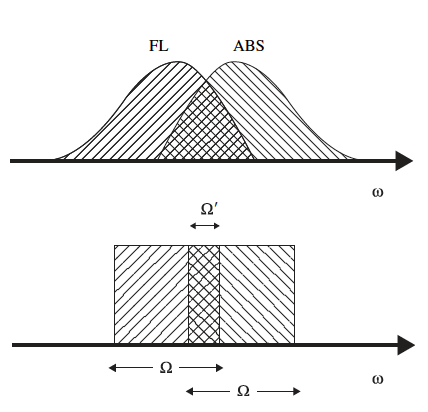
\includegraphics[width=0.6\textwidth]{capitulo2/overlap}
\caption{\small{Espectros de emisi\'on y absorci\'on de intensidad vs frecuencia, $\Omega'$ representa el ancho de la superposici\'on}\label{integral}}   
\end{figure}


La eficiencia de transferencia de energ\'ia de resonanacia F\"orster $E$ se define como la fracci\'on de fotones que son absorbidos por la mol\'ecula donadora y son transferidos a la mol\'ecula aceptora, o bien:

\begin{align}
E=\frac{1}{1+(R/R_0)^6}
\end{align}

F\"orster asumi\'o que el proceso de transferencia de energ\'ia no radiativa es mucho m\'as lento que la relajaci\'on vibracional entre los modos vibracionales del estado excitado debido a interacciones con el disolvente y determin\'o que la raz\'on de la transferencia de energ\'ia de resonancia $k_{D-A}$ puede expresarse como $k_{D-A}=\frac{1}{\tau_D} (\frac{R_0}{R})^6$, donde $\tau_D$ es el tiempo de vida medio de la mol\'ecula donadora en el estado excitado. 

La consideraci\'on de un acoplamiento d\'ebil entre dos osciladores: la mol\'ecula donadora y aceptora; o bien, de una interacci\'on d\'ebil de tipo dipolo--dipolo en la transferencia de energ\'ia de resonancia F\"orster, es lo que induce una transferencia de energ\'ia no radiativa e implica que las propiedades espectrales de la mol\'ecula donadora o aceptora no se vean afectadas \cite{megalibro}.

La t\'ecnica FRET se ha vuelto muy popular en estudios de biolog\'ia y qu\'imica, principalmente aplicada a microscop\'ia \'optica utilizando fluor\'oforos, ya que permite estudiar interacciones moleculares e interacciones entre pares de prote\'inas en c\'elulas vivas determinando las distancias que hay entre los sistemas donador y aceptor. En la mayor\'ia de aplicaciones la transferencia de energ\'ia de resonancia F\"orster se manifiesta en la disminuci\'on tanto del tiempo de vida como de la intensidad de fluorescencia del sistema donador acompa\~{n}ada de un incremento en la emisi\'on de fluorescencia del sistema aceptor.

%La transferencia de energ\'ia de resonancia F\"orster se puede presentar entre pares de \'atomos, mol\'eculas y agregados moleculares \cite{megalibro}.

